
\section{Introduction}

One of the major trends in city planning is the introduction of light rail transit networks. However, when spatial development was previously based on the automobile, the often low densities of residences and activities might not fit ideal conditions for a transit line. In order to ease the integration of a new transit line in the existing road network, one common idea is to include park and ride facilities around transit stations, allowing car-based access to the transit line.

Sioux Falls, South Dakota, is a city that has been experiencing rapid growth in recent years. The city, which still had a population of 125 000 at the start of the century, now has a population of over 200 000 in a superficy of 210 km$^2$\footnote{\url{https://en.wikipedia.org/wiki/Sioux_Falls,_South_Dakota}}. In population, this is comparable to the city of Geneva, which has multiple light transit lines, suburban train lines and a dense bus network (altough for a superficy of only 16 km$^2$\footnote{\url{https://fr.wikipedia.org/wiki/Gen\%C3\%A8ve}}). In comparison, Sioux Falls' public transport relies only on 9 bus lines, running only 6 days a week, and on-demand transport\footnote{\url{https://siouxareametro.info/bus}}. Additionally, Sioux Falls' road network inspired the homonymous benchmark network, which is well-known in traffic engineering for its small size and typical grid structure.

\begin{figure}
    \centering
    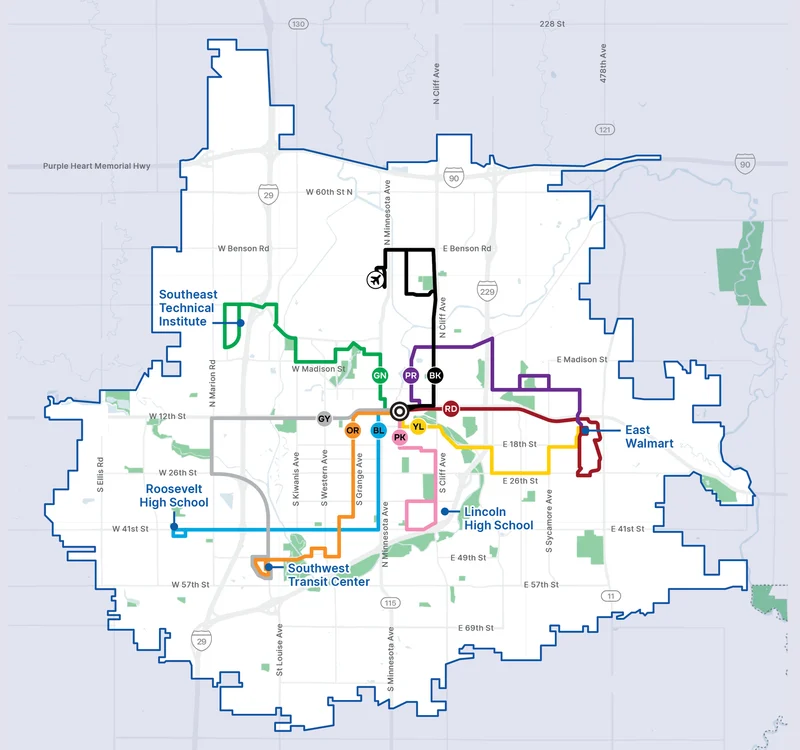
\includegraphics[keepaspectratio,width=0.45\textwidth]{Figures/siouxfalls_bus_network.png}
    \caption{Sioux Falls' current bus network.}
    \label{fig:sioux_falls_bus_network}
\end{figure}


In a hypothetical scenario, the city of Sioux Falls is considering the construction of a light rail line to improve public transport usage. This study will analyse the potential decrease in traffic of converting one existing bus lines into a light rail line, as well as the introduction of park and ride facilities at the stations. In order to do that, we will solve the trafic at \textit{User Equilibrium} (UE) in the benchmark network, and then simulate the introduction of the new light rail line as new links between the nodes, with the restriction that one user might use it only if both its destination and its origin is along the line. Finally, the introduction of park and ride facilities will be simulated by replacing the previous constraint, and allowing users to access the light rail line if one of their origin or destination is along the line. 

Future research could consider parking and ticket fares, the inconvenience of having to change mode and the waiting time to be included in a generic cost added to the travel time on the transit line. The possibility to only include park and ride facilities at only some stations, limit the capacity of the parkings, more sensitive cost computation (e.g. precise computation, inclusion of fuel cost in individual transport links) and a sensibility analysis on the value of the generic cost would, if time allows, be interesting to include in the study.


The project would be done individually.